\documentclass[1p]{elsarticle_modified}
%\bibliographystyle{elsarticle-num}

%\usepackage[colorlinks]{hyperref}
%\usepackage{abbrmath_seonhwa} %\Abb, \Ascr, \Acal ,\Abf, \Afrak
\usepackage{amsfonts}
\usepackage{amssymb}
\usepackage{amsmath}
\usepackage{amsthm}
\usepackage{scalefnt}
\usepackage{amsbsy}
\usepackage{kotex}
\usepackage{caption}
\usepackage{subfig}
\usepackage{color}
\usepackage{graphicx}
\usepackage{xcolor} %% white, black, red, green, blue, cyan, magenta, yellow
\usepackage{float}
\usepackage{setspace}
\usepackage{hyperref}

\usepackage{tikz}
\usetikzlibrary{arrows}

\usepackage{multirow}
\usepackage{array} % fixed length table
\usepackage{hhline}

%%%%%%%%%%%%%%%%%%%%%
\makeatletter
\renewcommand*\env@matrix[1][\arraystretch]{%
	\edef\arraystretch{#1}%
	\hskip -\arraycolsep
	\let\@ifnextchar\new@ifnextchar
	\array{*\c@MaxMatrixCols c}}
\makeatother %https://tex.stackexchange.com/questions/14071/how-can-i-increase-the-line-spacing-in-a-matrix
%%%%%%%%%%%%%%%

\usepackage[normalem]{ulem}

\newcommand{\msout}[1]{\ifmmode\text{\sout{\ensuremath{#1}}}\else\sout{#1}\fi}
%SOURCE: \msout is \stkout macro in https://tex.stackexchange.com/questions/20609/strikeout-in-math-mode

\newcommand{\cancel}[1]{
	\ifmmode
	{\color{red}\msout{#1}}
	\else
	{\color{red}\sout{#1}}
	\fi
}

\newcommand{\add}[1]{
	{\color{blue}\uwave{#1}}
}

\newcommand{\replace}[2]{
	\ifmmode
	{\color{red}\msout{#1}}{\color{blue}\uwave{#2}}
	\else
	{\color{red}\sout{#1}}{\color{blue}\uwave{#2}}
	\fi
}

\newcommand{\Sol}{\mathcal{S}} %segment
\newcommand{\D}{D} %diagram
\newcommand{\A}{\mathcal{A}} %arc


%%%%%%%%%%%%%%%%%%%%%%%%%%%%%5 test

\def\sl{\operatorname{\textup{SL}}(2,\Cbb)}
\def\psl{\operatorname{\textup{PSL}}(2,\Cbb)}
\def\quan{\mkern 1mu \triangleright \mkern 1mu}

\theoremstyle{definition}
\newtheorem{thm}{Theorem}[section]
\newtheorem{prop}[thm]{Proposition}
\newtheorem{lem}[thm]{Lemma}
\newtheorem{ques}[thm]{Question}
\newtheorem{cor}[thm]{Corollary}
\newtheorem{defn}[thm]{Definition}
\newtheorem{exam}[thm]{Example}
\newtheorem{rmk}[thm]{Remark}
\newtheorem{alg}[thm]{Algorithm}

\newcommand{\I}{\sqrt{-1}}
\begin{document}

%\begin{frontmatter}
%
%\title{Boundary parabolic representations of knots up to 8 crossings}
%
%%% Group authors per affiliation:
%\author{Yunhi Cho} 
%\address{Department of Mathematics, University of Seoul, Seoul, Korea}
%\ead{yhcho@uos.ac.kr}
%
%
%\author{Seonhwa Kim} %\fnref{s_kim}}
%\address{Center for Geometry and Physics, Institute for Basic Science, Pohang, 37673, Korea}
%\ead{ryeona17@ibs.re.kr}
%
%\author{Hyuk Kim}
%\address{Department of Mathematical Sciences, Seoul National University, Seoul 08826, Korea}
%\ead{hyukkim@snu.ac.kr}
%
%\author{Seokbeom Yoon}
%\address{Department of Mathematical Sciences, Seoul National University, Seoul, 08826,  Korea}
%\ead{sbyoon15@snu.ac.kr}
%
%\begin{abstract}
%We find all boundary parabolic representation of knots up to 8 crossings.
%
%\end{abstract}
%\begin{keyword}
%    \MSC[2010] 57M25 
%\end{keyword}
%
%\end{frontmatter}

%\linenumbers
%\tableofcontents
%
\newcommand\colored[1]{\textcolor{white}{\rule[-0.35ex]{0.8em}{1.4ex}}\kern-0.8em\color{red} #1}%
%\newcommand\colored[1]{\textcolor{white}{ #1}\kern-2.17ex	\textcolor{white}{ #1}\kern-1.81ex	\textcolor{white}{ #1}\kern-2.15ex\color{red}#1	}

{\Large $\underline{12a_{0365}~(K12a_{0365})}$}

\setlength{\tabcolsep}{10pt}
\renewcommand{\arraystretch}{1.6}
\vspace{1cm}\begin{tabular}{m{100pt}>{\centering\arraybackslash}m{274pt}}
\multirow{5}{120pt}{
	\centering
	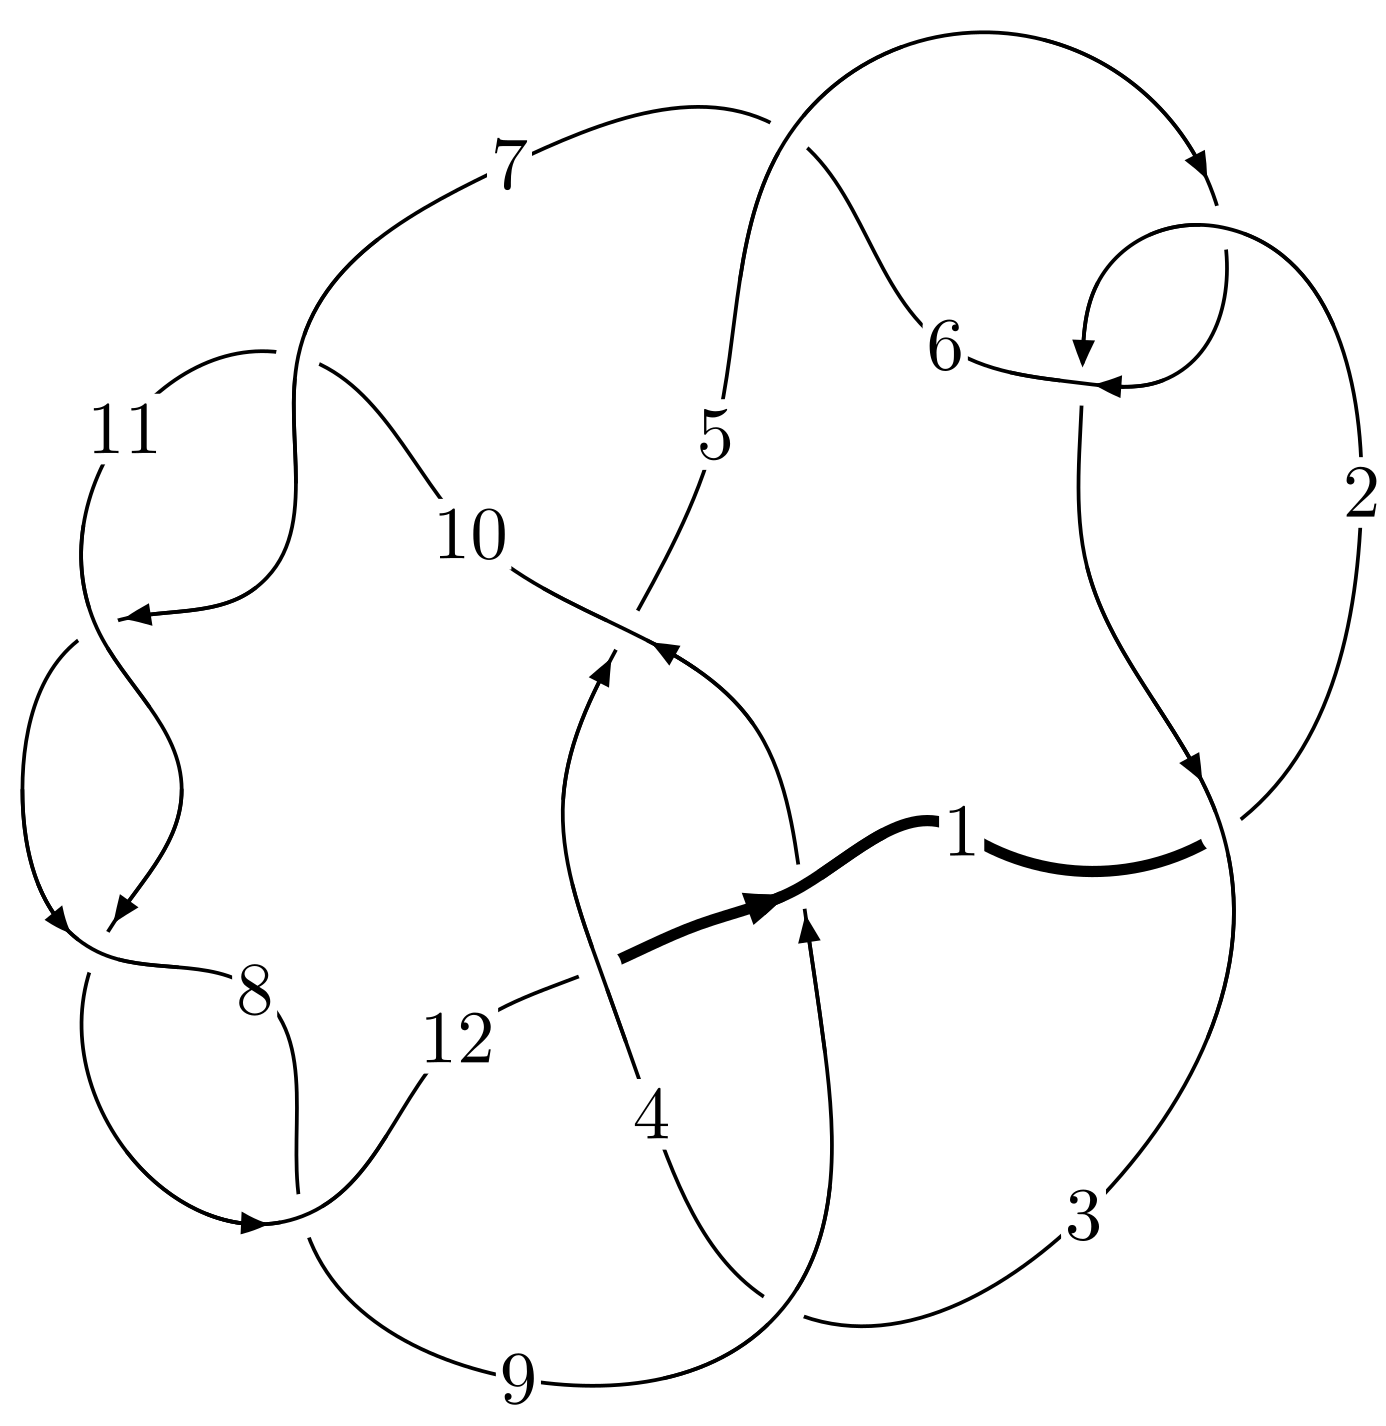
\includegraphics[width=112pt]{../../../GIT/diagram.site/Diagrams/png/1166_12a_0365.png}\\
\ \ \ A knot diagram\footnotemark}&
\allowdisplaybreaks
\textbf{Linearized knot diagam} \\
\cline{2-2}
 &
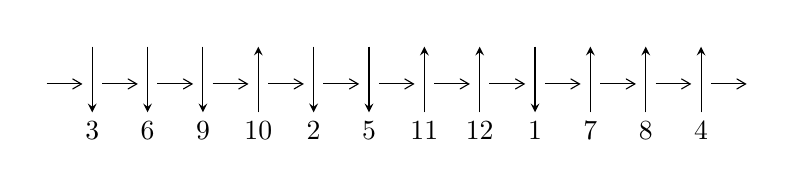
\begin{tikzpicture}[x=20pt, y=17pt]
	% nodes
	\node (C0) at (0, 0) {};
	\node (C1) at (1, 0) {};
	\node (C1U) at (1, +1) {};
	\node (C1D) at (1, -1) {3};

	\node (C2) at (2, 0) {};
	\node (C2U) at (2, +1) {};
	\node (C2D) at (2, -1) {6};

	\node (C3) at (3, 0) {};
	\node (C3U) at (3, +1) {};
	\node (C3D) at (3, -1) {9};

	\node (C4) at (4, 0) {};
	\node (C4U) at (4, +1) {};
	\node (C4D) at (4, -1) {10};

	\node (C5) at (5, 0) {};
	\node (C5U) at (5, +1) {};
	\node (C5D) at (5, -1) {2};

	\node (C6) at (6, 0) {};
	\node (C6U) at (6, +1) {};
	\node (C6D) at (6, -1) {5};

	\node (C7) at (7, 0) {};
	\node (C7U) at (7, +1) {};
	\node (C7D) at (7, -1) {11};

	\node (C8) at (8, 0) {};
	\node (C8U) at (8, +1) {};
	\node (C8D) at (8, -1) {12};

	\node (C9) at (9, 0) {};
	\node (C9U) at (9, +1) {};
	\node (C9D) at (9, -1) {1};

	\node (C10) at (10, 0) {};
	\node (C10U) at (10, +1) {};
	\node (C10D) at (10, -1) {7};

	\node (C11) at (11, 0) {};
	\node (C11U) at (11, +1) {};
	\node (C11D) at (11, -1) {8};

	\node (C12) at (12, 0) {};
	\node (C12U) at (12, +1) {};
	\node (C12D) at (12, -1) {4};
	\node (C13) at (13, 0) {};

	% arrows
	\draw[->,>={angle 60}]
	(C0) edge (C1) (C1) edge (C2) (C2) edge (C3) (C3) edge (C4) (C4) edge (C5) (C5) edge (C6) (C6) edge (C7) (C7) edge (C8) (C8) edge (C9) (C9) edge (C10) (C10) edge (C11) (C11) edge (C12) (C12) edge (C13) ;	\draw[->,>=stealth]
	(C1U) edge (C1D) (C2U) edge (C2D) (C3U) edge (C3D) (C4D) edge (C4U) (C5U) edge (C5D) (C6U) edge (C6D) (C7D) edge (C7U) (C8D) edge (C8U) (C9U) edge (C9D) (C10D) edge (C10U) (C11D) edge (C11U) (C12D) edge (C12U) ;
	\end{tikzpicture} \\
\hhline{~~} \\& 
\textbf{Solving Sequence} \\ \cline{2-2} 
 &
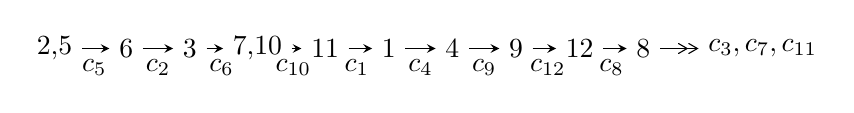
\begin{tikzpicture}[x=23pt, y=7pt]
	% node
	\node (A0) at (-1/8, 0) {2,5};
	\node (A1) at (1, 0) {6};
	\node (A2) at (2, 0) {3};
	\node (A3) at (49/16, 0) {7,10};
	\node (A4) at (33/8, 0) {11};
	\node (A5) at (41/8, 0) {1};
	\node (A6) at (49/8, 0) {4};
	\node (A7) at (57/8, 0) {9};
	\node (A8) at (65/8, 0) {12};
	\node (A9) at (73/8, 0) {8};
	\node (C1) at (1/2, -1) {$c_{5}$};
	\node (C2) at (3/2, -1) {$c_{2}$};
	\node (C3) at (5/2, -1) {$c_{6}$};
	\node (C4) at (29/8, -1) {$c_{10}$};
	\node (C5) at (37/8, -1) {$c_{1}$};
	\node (C6) at (45/8, -1) {$c_{4}$};
	\node (C7) at (53/8, -1) {$c_{9}$};
	\node (C8) at (61/8, -1) {$c_{12}$};
	\node (C9) at (69/8, -1) {$c_{8}$};
	\node (A10) at (11, 0) {$c_{3},c_{7},c_{11}$};

	% edge
	\draw[->,>=stealth]	
	(A0) edge (A1) (A1) edge (A2) (A2) edge (A3) (A3) edge (A4) (A4) edge (A5) (A5) edge (A6) (A6) edge (A7) (A7) edge (A8) (A8) edge (A9) ;
	\draw[->>,>={angle 60}]	
	(A9) edge (A10);
\end{tikzpicture} \\ 

\end{tabular} \\

\footnotetext{
The image of knot diagram is generated by the software ``\textbf{Draw programme}" developed by Andrew Bartholomew(\url{http://www.layer8.co.uk/maths/draw/index.htm\#Running-draw}), where we modified some parts for our purpose(\url{https://github.com/CATsTAILs/LinksPainter}).
}\phantom \\ \newline 
\centering \textbf{Ideals for irreducible components\footnotemark of $X_{\text{par}}$} 
 
\begin{align*}
I^u_{1}&=\langle 
5.12893\times10^{45} u^{69}+1.68277\times10^{46} u^{68}+\cdots+4.63662\times10^{44} b-6.98652\times10^{45},\\
\phantom{I^u_{1}}&\phantom{= \langle  }5.16448\times10^{45} u^{69}+1.76696\times10^{46} u^{68}+\cdots+4.63662\times10^{44} a-1.03706\times10^{46},\;u^{70}+4 u^{69}+\cdots+9 u-1\rangle \\
I^u_{2}&=\langle 
u^2+b,\;- u^2+a+u,\;u^3- u^2+1\rangle \\
I^u_{3}&=\langle 
b- a,\;a^2+a-1,\;u+1\rangle \\
\\
\end{align*}
\raggedright * 3 irreducible components of $\dim_{\mathbb{C}}=0$, with total 75 representations.\\
\footnotetext{All coefficients of polynomials are rational numbers. But the coefficients are sometimes approximated in decimal forms when there is not enough margin.}
\newpage
\renewcommand{\arraystretch}{1}
\centering \section*{I. $I^u_{1}= \langle 5.13\times10^{45} u^{69}+1.68\times10^{46} u^{68}+\cdots+4.64\times10^{44} b-6.99\times10^{45},\;5.16\times10^{45} u^{69}+1.77\times10^{46} u^{68}+\cdots+4.64\times10^{44} a-1.04\times10^{46},\;u^{70}+4 u^{69}+\cdots+9 u-1 \rangle$}
\flushleft \textbf{(i) Arc colorings}\\
\begin{tabular}{m{7pt} m{180pt} m{7pt} m{180pt} }
\flushright $a_{2}=$&$\begin{pmatrix}0\\u\end{pmatrix}$ \\
\flushright $a_{5}=$&$\begin{pmatrix}1\\0\end{pmatrix}$ \\
\flushright $a_{6}=$&$\begin{pmatrix}1\\u^2\end{pmatrix}$ \\
\flushright $a_{3}=$&$\begin{pmatrix}- u\\- u^3+u\end{pmatrix}$ \\
\flushright $a_{7}=$&$\begin{pmatrix}- u^2+1\\u^2\end{pmatrix}$ \\
\flushright $a_{10}=$&$\begin{pmatrix}-11.1385 u^{69}-38.1088 u^{68}+\cdots-173.343 u+22.3667\\-11.0618 u^{69}-36.2931 u^{68}+\cdots-165.547 u+15.0681\end{pmatrix}$ \\
\flushright $a_{11}=$&$\begin{pmatrix}-10.4892 u^{69}-34.4257 u^{68}+\cdots-156.393 u+19.8877\\-14.0832 u^{69}-46.3168 u^{68}+\cdots-196.252 u+18.2161\end{pmatrix}$ \\
\flushright $a_{1}=$&$\begin{pmatrix}u^3\\u^5- u^3+u\end{pmatrix}$ \\
\flushright $a_{4}=$&$\begin{pmatrix}-3.13298 u^{69}-9.84215 u^{68}+\cdots-17.5436 u-1.28092\\1.91095 u^{69}+6.30251 u^{68}+\cdots+32.7284 u-2.47449\end{pmatrix}$ \\
\flushright $a_{9}=$&$\begin{pmatrix}-9.64324 u^{69}-30.9560 u^{68}+\cdots-143.863 u+19.4560\\-13.0842 u^{69}-43.4668 u^{68}+\cdots-180.730 u+16.7111\end{pmatrix}$ \\
\flushright $a_{12}=$&$\begin{pmatrix}4.89906 u^{69}+16.4905 u^{68}+\cdots+65.1053 u-7.37396\\4.33074 u^{69}+13.3350 u^{68}+\cdots+61.2047 u-5.58668\end{pmatrix}$ \\
\flushright $a_{8}=$&$\begin{pmatrix}-4.02982 u^{69}-12.7973 u^{68}+\cdots-53.5338 u+10.0666\\-3.38116 u^{69}-10.7655 u^{68}+\cdots-42.5744 u+3.57024\end{pmatrix}$\\&\end{tabular}
\flushleft \textbf{(ii) Obstruction class $= -1$}\\~\\
\flushleft \textbf{(iii) Cusp Shapes $= -128.394 u^{69}-417.002 u^{68}+\cdots-1794.20 u+180.894$}\\~\\
\newpage\renewcommand{\arraystretch}{1}
\flushleft \textbf{(iv) u-Polynomials at the component}\newline \\
\begin{tabular}{m{50pt}|m{274pt}}
Crossings & \hspace{64pt}u-Polynomials at each crossing \\
\hline $$\begin{aligned}c_{1},c_{6}\end{aligned}$$&$\begin{aligned}
&u^{70}+20 u^{69}+\cdots+85 u+1
\end{aligned}$\\
\hline $$\begin{aligned}c_{2},c_{5}\end{aligned}$$&$\begin{aligned}
&u^{70}+4 u^{69}+\cdots+9 u-1
\end{aligned}$\\
\hline $$\begin{aligned}c_{3}\end{aligned}$$&$\begin{aligned}
&u^{70}-3 u^{69}+\cdots-1882 u-203
\end{aligned}$\\
\hline $$\begin{aligned}c_{4}\end{aligned}$$&$\begin{aligned}
&u^{70}- u^{69}+\cdots-1480438 u-582613
\end{aligned}$\\
\hline $$\begin{aligned}c_{7},c_{8},c_{10}\\c_{11}\end{aligned}$$&$\begin{aligned}
&u^{70}-5 u^{69}+\cdots-5 u-1
\end{aligned}$\\
\hline $$\begin{aligned}c_{9}\end{aligned}$$&$\begin{aligned}
&u^{70}+4 u^{69}+\cdots+8 u+4
\end{aligned}$\\
\hline $$\begin{aligned}c_{12}\end{aligned}$$&$\begin{aligned}
&u^{70}+7 u^{69}+\cdots+20 u+8
\end{aligned}$\\
\hline
\end{tabular}\\~\\
\newpage\renewcommand{\arraystretch}{1}
\flushleft \textbf{(v) Riley Polynomials at the component}\newline \\
\begin{tabular}{m{50pt}|m{274pt}}
Crossings & \hspace{64pt}Riley Polynomials at each crossing \\
\hline $$\begin{aligned}c_{1},c_{6}\end{aligned}$$&$\begin{aligned}
&y^{70}+64 y^{69}+\cdots-5893 y+1
\end{aligned}$\\
\hline $$\begin{aligned}c_{2},c_{5}\end{aligned}$$&$\begin{aligned}
&y^{70}-20 y^{69}+\cdots-85 y+1
\end{aligned}$\\
\hline $$\begin{aligned}c_{3}\end{aligned}$$&$\begin{aligned}
&y^{70}+99 y^{69}+\cdots+1211930 y+41209
\end{aligned}$\\
\hline $$\begin{aligned}c_{4}\end{aligned}$$&$\begin{aligned}
&y^{70}+27 y^{69}+\cdots-15150651595278 y+339437907769
\end{aligned}$\\
\hline $$\begin{aligned}c_{7},c_{8},c_{10}\\c_{11}\end{aligned}$$&$\begin{aligned}
&y^{70}-87 y^{69}+\cdots-151 y+1
\end{aligned}$\\
\hline $$\begin{aligned}c_{9}\end{aligned}$$&$\begin{aligned}
&y^{70}+12 y^{69}+\cdots+184 y+16
\end{aligned}$\\
\hline $$\begin{aligned}c_{12}\end{aligned}$$&$\begin{aligned}
&y^{70}-23 y^{69}+\cdots+176 y+64
\end{aligned}$\\
\hline
\end{tabular}\\~\\
\newpage\flushleft \textbf{(vi) Complex Volumes and Cusp Shapes}
$$\begin{array}{c|c|c}  
\text{Solutions to }I^u_{1}& \I (\text{vol} + \sqrt{-1}CS) & \text{Cusp shape}\\
 \hline 
\begin{aligned}
u &= -0.821992 + 0.604536 I \\
a &= -0.532818 + 0.414673 I \\
b &= -0.120277 + 1.017190 I\end{aligned}
 & \phantom{-}3.21297 + 2.35752 I & \phantom{-0.000000 } 0 \\ \hline\begin{aligned}
u &= -0.821992 - 0.604536 I \\
a &= -0.532818 - 0.414673 I \\
b &= -0.120277 - 1.017190 I\end{aligned}
 & \phantom{-}3.21297 - 2.35752 I & \phantom{-0.000000 } 0 \\ \hline\begin{aligned}
u &= \phantom{-}0.936330 + 0.264637 I \\
a &= -0.896597 - 0.840149 I \\
b &= \phantom{-}0.665791 - 0.751664 I\end{aligned}
 & -2.22755 - 3.95507 I & \phantom{-0.000000 } 0 \\ \hline\begin{aligned}
u &= \phantom{-}0.936330 - 0.264637 I \\
a &= -0.896597 + 0.840149 I \\
b &= \phantom{-}0.665791 + 0.751664 I\end{aligned}
 & -2.22755 + 3.95507 I & \phantom{-0.000000 } 0 \\ \hline\begin{aligned}
u &= -0.894877 + 0.344146 I \\
a &= \phantom{-}0.584785 - 0.204131 I \\
b &= \phantom{-}0.118346 - 0.802002 I\end{aligned}
 & -1.90739 + 1.11321 I & \phantom{-0.000000 } 0 \\ \hline\begin{aligned}
u &= -0.894877 - 0.344146 I \\
a &= \phantom{-}0.584785 + 0.204131 I \\
b &= \phantom{-}0.118346 + 0.802002 I\end{aligned}
 & -1.90739 - 1.11321 I & \phantom{-0.000000 } 0 \\ \hline\begin{aligned}
u &= \phantom{-}0.853926 + 0.379140 I \\
a &= -1.07991 + 2.13533 I \\
b &= -0.768766 - 0.133800 I\end{aligned}
 & \phantom{-}8.86997 - 3.71004 I & \phantom{-}5.02992 + 4.95815 I \\ \hline\begin{aligned}
u &= \phantom{-}0.853926 - 0.379140 I \\
a &= -1.07991 - 2.13533 I \\
b &= -0.768766 + 0.133800 I\end{aligned}
 & \phantom{-}8.86997 + 3.71004 I & \phantom{-}5.02992 - 4.95815 I \\ \hline\begin{aligned}
u &= \phantom{-}0.076050 + 0.910271 I \\
a &= \phantom{-}0.786878 + 0.417494 I \\
b &= -1.286790 - 0.266397 I\end{aligned}
 & \phantom{-}12.21590 + 5.26874 I & \phantom{-}9.05075 - 4.23813 I \\ \hline\begin{aligned}
u &= \phantom{-}0.076050 - 0.910271 I \\
a &= \phantom{-}0.786878 - 0.417494 I \\
b &= -1.286790 + 0.266397 I\end{aligned}
 & \phantom{-}12.21590 - 5.26874 I & \phantom{-}9.05075 + 4.23813 I\\
 \hline 
 \end{array}$$\newpage$$\begin{array}{c|c|c}  
\text{Solutions to }I^u_{1}& \I (\text{vol} + \sqrt{-1}CS) & \text{Cusp shape}\\
 \hline 
\begin{aligned}
u &= \phantom{-}1.053090 + 0.329534 I \\
a &= \phantom{-}0.301987 + 0.839033 I \\
b &= -0.884319 + 0.768012 I\end{aligned}
 & \phantom{-}0.05205 - 7.60424 I & \phantom{-0.000000 } 0 \\ \hline\begin{aligned}
u &= \phantom{-}1.053090 - 0.329534 I \\
a &= \phantom{-}0.301987 - 0.839033 I \\
b &= -0.884319 - 0.768012 I\end{aligned}
 & \phantom{-}0.05205 + 7.60424 I & \phantom{-0.000000 } 0 \\ \hline\begin{aligned}
u &= -0.873719\phantom{ +0.000000I} \\
a &= \phantom{-}0.0354661\phantom{ +0.000000I} \\
b &= \phantom{-}0.465987\phantom{ +0.000000I}\end{aligned}
 & -1.43825\phantom{ +0.000000I} & -7.21730\phantom{ +0.000000I} \\ \hline\begin{aligned}
u &= \phantom{-}0.839383 + 0.766541 I \\
a &= \phantom{-}1.97243 + 0.15164 I \\
b &= -1.28254 + 0.70957 I\end{aligned}
 & \phantom{-}3.50192 - 1.96491 I & \phantom{-0.000000 } 0 \\ \hline\begin{aligned}
u &= \phantom{-}0.839383 - 0.766541 I \\
a &= \phantom{-}1.97243 - 0.15164 I \\
b &= -1.28254 - 0.70957 I\end{aligned}
 & \phantom{-}3.50192 + 1.96491 I & \phantom{-0.000000 } 0 \\ \hline\begin{aligned}
u &= -1.130380 + 0.210061 I \\
a &= -0.464632 - 0.272711 I \\
b &= -0.451919 + 0.228098 I\end{aligned}
 & -0.745084 - 0.635310 I & \phantom{-0.000000 } 0 \\ \hline\begin{aligned}
u &= -1.130380 - 0.210061 I \\
a &= -0.464632 + 0.272711 I \\
b &= -0.451919 - 0.228098 I\end{aligned}
 & -0.745084 + 0.635310 I & \phantom{-0.000000 } 0 \\ \hline\begin{aligned}
u &= \phantom{-}0.879194 + 0.755731 I \\
a &= -2.58309 + 2.90548 I \\
b &= -0.13084 - 3.76242 I\end{aligned}
 & \phantom{-}4.28859 - 2.86154 I & \phantom{-0.000000 } 0 \\ \hline\begin{aligned}
u &= \phantom{-}0.879194 - 0.755731 I \\
a &= -2.58309 - 2.90548 I \\
b &= -0.13084 + 3.76242 I\end{aligned}
 & \phantom{-}4.28859 + 2.86154 I & \phantom{-0.000000 } 0 \\ \hline\begin{aligned}
u &= -0.818848 + 0.830702 I \\
a &= \phantom{-}1.51994 - 0.93351 I \\
b &= -1.068180 + 0.239833 I\end{aligned}
 & \phantom{-}4.67474 - 1.95463 I & \phantom{-0.000000 } 0\\
 \hline 
 \end{array}$$\newpage$$\begin{array}{c|c|c}  
\text{Solutions to }I^u_{1}& \I (\text{vol} + \sqrt{-1}CS) & \text{Cusp shape}\\
 \hline 
\begin{aligned}
u &= -0.818848 - 0.830702 I \\
a &= \phantom{-}1.51994 + 0.93351 I \\
b &= -1.068180 - 0.239833 I\end{aligned}
 & \phantom{-}4.67474 + 1.95463 I & \phantom{-0.000000 } 0 \\ \hline\begin{aligned}
u &= \phantom{-}0.756256 + 0.888290 I \\
a &= -0.908087 - 0.235986 I \\
b &= \phantom{-}0.978137 + 0.193385 I\end{aligned}
 & \phantom{-}7.15283 - 0.79673 I & \phantom{-0.000000 } 0 \\ \hline\begin{aligned}
u &= \phantom{-}0.756256 - 0.888290 I \\
a &= -0.908087 + 0.235986 I \\
b &= \phantom{-}0.978137 - 0.193385 I\end{aligned}
 & \phantom{-}7.15283 + 0.79673 I & \phantom{-0.000000 } 0 \\ \hline\begin{aligned}
u &= -0.779738 + 0.882642 I \\
a &= -1.34956 + 0.96896 I \\
b &= \phantom{-}1.40703 - 0.65492 I\end{aligned}
 & \phantom{-}8.05847 - 6.46660 I & \phantom{-0.000000 } 0 \\ \hline\begin{aligned}
u &= -0.779738 - 0.882642 I \\
a &= -1.34956 - 0.96896 I \\
b &= \phantom{-}1.40703 + 0.65492 I\end{aligned}
 & \phantom{-}8.05847 + 6.46660 I & \phantom{-0.000000 } 0 \\ \hline\begin{aligned}
u &= \phantom{-}0.921897 + 0.750500 I \\
a &= -1.04326 - 1.35120 I \\
b &= \phantom{-}1.282040 + 0.357501 I\end{aligned}
 & \phantom{-}3.24664 - 3.77981 I & \phantom{-0.000000 } 0 \\ \hline\begin{aligned}
u &= \phantom{-}0.921897 - 0.750500 I \\
a &= -1.04326 + 1.35120 I \\
b &= \phantom{-}1.282040 - 0.357501 I\end{aligned}
 & \phantom{-}3.24664 + 3.77981 I & \phantom{-0.000000 } 0 \\ \hline\begin{aligned}
u &= \phantom{-}0.890245 + 0.790410 I \\
a &= \phantom{-}2.42222 - 2.22983 I \\
b &= \phantom{-}0.02417 + 3.67851 I\end{aligned}
 & \phantom{-}12.73530 - 2.97097 I & \phantom{-0.000000 } 0 \\ \hline\begin{aligned}
u &= \phantom{-}0.890245 - 0.790410 I \\
a &= \phantom{-}2.42222 + 2.22983 I \\
b &= \phantom{-}0.02417 - 3.67851 I\end{aligned}
 & \phantom{-}12.73530 + 2.97097 I & \phantom{-0.000000 } 0 \\ \hline\begin{aligned}
u &= -0.795789 + 0.142506 I \\
a &= -1.53396 - 2.52646 I \\
b &= -1.17773 - 2.40528 I\end{aligned}
 & \phantom{-}7.52169 + 0.34716 I & \phantom{-}21.0536 + 3.3715 I\\
 \hline 
 \end{array}$$\newpage$$\begin{array}{c|c|c}  
\text{Solutions to }I^u_{1}& \I (\text{vol} + \sqrt{-1}CS) & \text{Cusp shape}\\
 \hline 
\begin{aligned}
u &= -0.795789 - 0.142506 I \\
a &= -1.53396 + 2.52646 I \\
b &= -1.17773 + 2.40528 I\end{aligned}
 & \phantom{-}7.52169 - 0.34716 I & \phantom{-}21.0536 - 3.3715 I \\ \hline\begin{aligned}
u &= \phantom{-}1.140890 + 0.364834 I \\
a &= \phantom{-}0.103618 - 0.905249 I \\
b &= \phantom{-}1.175310 - 0.699942 I\end{aligned}
 & \phantom{-}8.58977 - 9.64731 I & \phantom{-0.000000 } 0 \\ \hline\begin{aligned}
u &= \phantom{-}1.140890 - 0.364834 I \\
a &= \phantom{-}0.103618 + 0.905249 I \\
b &= \phantom{-}1.175310 + 0.699942 I\end{aligned}
 & \phantom{-}8.58977 + 9.64731 I & \phantom{-0.000000 } 0 \\ \hline\begin{aligned}
u &= -0.879597 + 0.814650 I \\
a &= -1.56862 + 1.07443 I \\
b &= \phantom{-}0.986495 + 0.292630 I\end{aligned}
 & \phantom{-}6.96123 + 3.17768 I & \phantom{-0.000000 } 0 \\ \hline\begin{aligned}
u &= -0.879597 - 0.814650 I \\
a &= -1.56862 - 1.07443 I \\
b &= \phantom{-}0.986495 - 0.292630 I\end{aligned}
 & \phantom{-}6.96123 - 3.17768 I & \phantom{-0.000000 } 0 \\ \hline\begin{aligned}
u &= -0.765989 + 0.932811 I \\
a &= \phantom{-}1.26151 - 1.07522 I \\
b &= -1.77664 + 0.92423 I\end{aligned}
 & \phantom{-}17.3945 - 9.1380 I & \phantom{-0.000000 } 0 \\ \hline\begin{aligned}
u &= -0.765989 - 0.932811 I \\
a &= \phantom{-}1.26151 + 1.07522 I \\
b &= -1.77664 - 0.92423 I\end{aligned}
 & \phantom{-}17.3945 + 9.1380 I & \phantom{-0.000000 } 0 \\ \hline\begin{aligned}
u &= -0.861076 + 0.848477 I \\
a &= -0.859319 + 0.438890 I \\
b &= \phantom{-}1.26257 - 0.76714 I\end{aligned}
 & \phantom{-}16.2859 - 0.4977 I & \phantom{-0.000000 } 0 \\ \hline\begin{aligned}
u &= -0.861076 - 0.848477 I \\
a &= -0.859319 - 0.438890 I \\
b &= \phantom{-}1.26257 + 0.76714 I\end{aligned}
 & \phantom{-}16.2859 + 0.4977 I & \phantom{-0.000000 } 0 \\ \hline\begin{aligned}
u &= -0.908549 + 0.804614 I \\
a &= \phantom{-}1.43278 - 0.30075 I \\
b &= -1.103350 + 0.163447 I\end{aligned}
 & \phantom{-}6.87034 + 2.88148 I & \phantom{-0.000000 } 0\\
 \hline 
 \end{array}$$\newpage$$\begin{array}{c|c|c}  
\text{Solutions to }I^u_{1}& \I (\text{vol} + \sqrt{-1}CS) & \text{Cusp shape}\\
 \hline 
\begin{aligned}
u &= -0.908549 - 0.804614 I \\
a &= \phantom{-}1.43278 + 0.30075 I \\
b &= -1.103350 - 0.163447 I\end{aligned}
 & \phantom{-}6.87034 - 2.88148 I & \phantom{-0.000000 } 0 \\ \hline\begin{aligned}
u &= \phantom{-}0.744970 + 0.985585 I \\
a &= \phantom{-}0.647817 + 0.473956 I \\
b &= -1.163770 - 0.687098 I\end{aligned}
 & \phantom{-}16.4531 - 0.4058 I & \phantom{-0.000000 } 0 \\ \hline\begin{aligned}
u &= \phantom{-}0.744970 - 0.985585 I \\
a &= \phantom{-}0.647817 - 0.473956 I \\
b &= -1.163770 + 0.687098 I\end{aligned}
 & \phantom{-}16.4531 + 0.4058 I & \phantom{-0.000000 } 0 \\ \hline\begin{aligned}
u &= \phantom{-}0.069642 + 0.760028 I \\
a &= -0.793095 - 0.598689 I \\
b &= \phantom{-}0.859741 + 0.405238 I\end{aligned}
 & \phantom{-}3.25439 + 3.89128 I & \phantom{-}8.22204 - 6.04817 I \\ \hline\begin{aligned}
u &= \phantom{-}0.069642 - 0.760028 I \\
a &= -0.793095 + 0.598689 I \\
b &= \phantom{-}0.859741 - 0.405238 I\end{aligned}
 & \phantom{-}3.25439 - 3.89128 I & \phantom{-}8.22204 + 6.04817 I \\ \hline\begin{aligned}
u &= -0.958273 + 0.787843 I \\
a &= -1.80471 + 0.55498 I \\
b &= \phantom{-}1.167160 + 0.384223 I\end{aligned}
 & \phantom{-}4.24350 + 8.00749 I & \phantom{-0.000000 } 0 \\ \hline\begin{aligned}
u &= -0.958273 - 0.787843 I \\
a &= -1.80471 - 0.55498 I \\
b &= \phantom{-}1.167160 - 0.384223 I\end{aligned}
 & \phantom{-}4.24350 - 8.00749 I & \phantom{-0.000000 } 0 \\ \hline\begin{aligned}
u &= -0.939681 + 0.820477 I \\
a &= \phantom{-}1.49590 - 1.03839 I \\
b &= -1.084500 - 0.834712 I\end{aligned}
 & \phantom{-}16.0406 + 6.7093 I & \phantom{-0.000000 } 0 \\ \hline\begin{aligned}
u &= -0.939681 - 0.820477 I \\
a &= \phantom{-}1.49590 + 1.03839 I \\
b &= -1.084500 + 0.834712 I\end{aligned}
 & \phantom{-}16.0406 - 6.7093 I & \phantom{-0.000000 } 0 \\ \hline\begin{aligned}
u &= \phantom{-}0.715806 + 0.197898 I \\
a &= \phantom{-}1.90591 + 0.45104 I \\
b &= -0.684371 + 0.426921 I\end{aligned}
 & \phantom{-}1.024240 - 0.486676 I & \phantom{-}5.73519 + 8.27485 I\\
 \hline 
 \end{array}$$\newpage$$\begin{array}{c|c|c}  
\text{Solutions to }I^u_{1}& \I (\text{vol} + \sqrt{-1}CS) & \text{Cusp shape}\\
 \hline 
\begin{aligned}
u &= \phantom{-}0.715806 - 0.197898 I \\
a &= \phantom{-}1.90591 - 0.45104 I \\
b &= -0.684371 - 0.426921 I\end{aligned}
 & \phantom{-}1.024240 + 0.486676 I & \phantom{-}5.73519 - 8.27485 I \\ \hline\begin{aligned}
u &= -0.731580 + 0.051178 I \\
a &= \phantom{-}0.44870 + 2.26858 I \\
b &= \phantom{-}0.01502 + 2.39231 I\end{aligned}
 & -0.138452 + 0.200334 I & \phantom{-}4.9583 + 27.7973 I \\ \hline\begin{aligned}
u &= -0.731580 - 0.051178 I \\
a &= \phantom{-}0.44870 - 2.26858 I \\
b &= \phantom{-}0.01502 - 2.39231 I\end{aligned}
 & -0.138452 - 0.200334 I & \phantom{-}4.9583 - 27.7973 I \\ \hline\begin{aligned}
u &= -1.250450 + 0.234036 I \\
a &= \phantom{-}0.590103 + 0.537183 I \\
b &= \phantom{-}0.859854 + 0.006608 I\end{aligned}
 & \phantom{-}7.57482 - 1.28932 I & \phantom{-0.000000 } 0 \\ \hline\begin{aligned}
u &= -1.250450 - 0.234036 I \\
a &= \phantom{-}0.590103 - 0.537183 I \\
b &= \phantom{-}0.859854 - 0.006608 I\end{aligned}
 & \phantom{-}7.57482 + 1.28932 I & \phantom{-0.000000 } 0 \\ \hline\begin{aligned}
u &= -1.001820 + 0.796995 I \\
a &= \phantom{-}1.91846 - 0.82073 I \\
b &= -1.44365 - 0.79366 I\end{aligned}
 & \phantom{-}7.3655 + 12.6957 I & \phantom{-0.000000 } 0 \\ \hline\begin{aligned}
u &= -1.001820 - 0.796995 I \\
a &= \phantom{-}1.91846 + 0.82073 I \\
b &= -1.44365 + 0.79366 I\end{aligned}
 & \phantom{-}7.3655 - 12.6957 I & \phantom{-0.000000 } 0 \\ \hline\begin{aligned}
u &= \phantom{-}1.012350 + 0.795855 I \\
a &= \phantom{-}1.031530 + 0.756442 I \\
b &= -0.955690 + 0.405302 I\end{aligned}
 & \phantom{-}6.36559 - 5.43747 I & \phantom{-0.000000 } 0 \\ \hline\begin{aligned}
u &= \phantom{-}1.012350 - 0.795855 I \\
a &= \phantom{-}1.031530 - 0.756442 I \\
b &= -0.955690 - 0.405302 I\end{aligned}
 & \phantom{-}6.36559 + 5.43747 I & \phantom{-0.000000 } 0 \\ \hline\begin{aligned}
u &= -1.033470 + 0.811620 I \\
a &= -1.97244 + 1.02030 I \\
b &= \phantom{-}1.74303 + 1.08840 I\end{aligned}
 & \phantom{-}16.5467 + 15.5606 I & \phantom{-0.000000 } 0\\
 \hline 
 \end{array}$$\newpage$$\begin{array}{c|c|c}  
\text{Solutions to }I^u_{1}& \I (\text{vol} + \sqrt{-1}CS) & \text{Cusp shape}\\
 \hline 
\begin{aligned}
u &= -1.033470 - 0.811620 I \\
a &= -1.97244 - 1.02030 I \\
b &= \phantom{-}1.74303 - 1.08840 I\end{aligned}
 & \phantom{-}16.5467 - 15.5606 I & \phantom{-0.000000 } 0 \\ \hline\begin{aligned}
u &= \phantom{-}0.597160 + 0.280730 I \\
a &= \phantom{-}0.35750 - 2.20071 I \\
b &= \phantom{-}0.268738 + 0.108233 I\end{aligned}
 & \phantom{-}1.24480 - 1.64965 I & \phantom{-}7.01663 + 7.54846 I \\ \hline\begin{aligned}
u &= \phantom{-}0.597160 - 0.280730 I \\
a &= \phantom{-}0.35750 + 2.20071 I \\
b &= \phantom{-}0.268738 - 0.108233 I\end{aligned}
 & \phantom{-}1.24480 + 1.64965 I & \phantom{-}7.01663 - 7.54846 I \\ \hline\begin{aligned}
u &= \phantom{-}1.069430 + 0.833772 I \\
a &= -1.142940 - 0.662361 I \\
b &= \phantom{-}1.013930 - 0.881403 I\end{aligned}
 & \phantom{-}15.4304 - 6.2393 I & \phantom{-0.000000 } 0 \\ \hline\begin{aligned}
u &= \phantom{-}1.069430 - 0.833772 I \\
a &= -1.142940 + 0.662361 I \\
b &= \phantom{-}1.013930 + 0.881403 I\end{aligned}
 & \phantom{-}15.4304 + 6.2393 I & \phantom{-0.000000 } 0 \\ \hline\begin{aligned}
u &= \phantom{-}0.345521 + 0.465734 I \\
a &= -1.78206 + 0.64019 I \\
b &= \phantom{-}1.51987 - 0.09297 I\end{aligned}
 & \phantom{-}10.36090 + 0.46448 I & \phantom{-}7.45738 + 2.55790 I \\ \hline\begin{aligned}
u &= \phantom{-}0.345521 - 0.465734 I \\
a &= -1.78206 - 0.64019 I \\
b &= \phantom{-}1.51987 + 0.09297 I\end{aligned}
 & \phantom{-}10.36090 - 0.46448 I & \phantom{-}7.45738 - 2.55790 I \\ \hline\begin{aligned}
u &= \phantom{-}0.049655 + 0.436764 I \\
a &= \phantom{-}1.29855 + 1.08613 I \\
b &= -0.333410 - 0.509182 I\end{aligned}
 & \phantom{-}0.274835 + 1.373660 I & \phantom{-}2.74778 - 4.32482 I \\ \hline\begin{aligned}
u &= \phantom{-}0.049655 - 0.436764 I \\
a &= \phantom{-}1.29855 - 1.08613 I \\
b &= -0.333410 + 0.509182 I\end{aligned}
 & \phantom{-}0.274835 - 1.373660 I & \phantom{-}2.74778 + 4.32482 I \\ \hline\begin{aligned}
u &= \phantom{-}0.114333\phantom{ +0.000000I} \\
a &= \phantom{-}5.43350\phantom{ +0.000000I} \\
b &= -0.726957\phantom{ +0.000000I}\end{aligned}
 & \phantom{-}1.36710\phantom{ +0.000000I} & \phantom{-}7.44230\phantom{ +0.000000I}\\
 \hline 
 \end{array}$$\newpage\newpage\renewcommand{\arraystretch}{1}
\centering \section*{II. $I^u_{2}= \langle u^2+b,\;- u^2+a+u,\;u^3- u^2+1 \rangle$}
\flushleft \textbf{(i) Arc colorings}\\
\begin{tabular}{m{7pt} m{180pt} m{7pt} m{180pt} }
\flushright $a_{2}=$&$\begin{pmatrix}0\\u\end{pmatrix}$ \\
\flushright $a_{5}=$&$\begin{pmatrix}1\\0\end{pmatrix}$ \\
\flushright $a_{6}=$&$\begin{pmatrix}1\\u^2\end{pmatrix}$ \\
\flushright $a_{3}=$&$\begin{pmatrix}- u\\- u^2+u+1\end{pmatrix}$ \\
\flushright $a_{7}=$&$\begin{pmatrix}- u^2+1\\u^2\end{pmatrix}$ \\
\flushright $a_{10}=$&$\begin{pmatrix}u^2- u\\- u^2\end{pmatrix}$ \\
\flushright $a_{11}=$&$\begin{pmatrix}2 u^2- u-1\\-2 u^2\end{pmatrix}$ \\
\flushright $a_{1}=$&$\begin{pmatrix}u^2-1\\- u^2\end{pmatrix}$ \\
\flushright $a_{4}=$&$\begin{pmatrix}u+1\\u^2- u-1\end{pmatrix}$ \\
\flushright $a_{9}=$&$\begin{pmatrix}2 u^2- u-1\\-2 u^2\end{pmatrix}$ \\
\flushright $a_{12}=$&$\begin{pmatrix}u^2-1\\- u^2\end{pmatrix}$ \\
\flushright $a_{8}=$&$\begin{pmatrix}u^2- u\\- u^2\end{pmatrix}$\\&\end{tabular}
\flushleft \textbf{(ii) Obstruction class $= 1$}\\~\\
\flushleft \textbf{(iii) Cusp Shapes $= -2 u^2+7 u+2$}\\~\\
\newpage\renewcommand{\arraystretch}{1}
\flushleft \textbf{(iv) u-Polynomials at the component}\newline \\
\begin{tabular}{m{50pt}|m{274pt}}
Crossings & \hspace{64pt}u-Polynomials at each crossing \\
\hline $$\begin{aligned}c_{1}\end{aligned}$$&$\begin{aligned}
&u^3- u^2+2 u-1
\end{aligned}$\\
\hline $$\begin{aligned}c_{2}\end{aligned}$$&$\begin{aligned}
&u^3+u^2-1
\end{aligned}$\\
\hline $$\begin{aligned}c_{3},c_{4},c_{6}\end{aligned}$$&$\begin{aligned}
&u^3+u^2+2 u+1
\end{aligned}$\\
\hline $$\begin{aligned}c_{5}\end{aligned}$$&$\begin{aligned}
&u^3- u^2+1
\end{aligned}$\\
\hline $$\begin{aligned}c_{7},c_{8},c_{9}\end{aligned}$$&$\begin{aligned}
&(u+1)^3
\end{aligned}$\\
\hline $$\begin{aligned}c_{10},c_{11}\end{aligned}$$&$\begin{aligned}
&(u-1)^3
\end{aligned}$\\
\hline $$\begin{aligned}c_{12}\end{aligned}$$&$\begin{aligned}
&u^3
\end{aligned}$\\
\hline
\end{tabular}\\~\\
\newpage\renewcommand{\arraystretch}{1}
\flushleft \textbf{(v) Riley Polynomials at the component}\newline \\
\begin{tabular}{m{50pt}|m{274pt}}
Crossings & \hspace{64pt}Riley Polynomials at each crossing \\
\hline $$\begin{aligned}c_{1},c_{3},c_{4}\\c_{6}\end{aligned}$$&$\begin{aligned}
&y^3+3 y^2+2 y-1
\end{aligned}$\\
\hline $$\begin{aligned}c_{2},c_{5}\end{aligned}$$&$\begin{aligned}
&y^3- y^2+2 y-1
\end{aligned}$\\
\hline $$\begin{aligned}c_{7},c_{8},c_{9}\\c_{10},c_{11}\end{aligned}$$&$\begin{aligned}
&(y-1)^3
\end{aligned}$\\
\hline $$\begin{aligned}c_{12}\end{aligned}$$&$\begin{aligned}
&y^3
\end{aligned}$\\
\hline
\end{tabular}\\~\\
\newpage\flushleft \textbf{(vi) Complex Volumes and Cusp Shapes}
$$\begin{array}{c|c|c}  
\text{Solutions to }I^u_{2}& \I (\text{vol} + \sqrt{-1}CS) & \text{Cusp shape}\\
 \hline 
\begin{aligned}
u &= \phantom{-}0.877439 + 0.744862 I \\
a &= -0.662359 + 0.562280 I \\
b &= -0.215080 - 1.307140 I\end{aligned}
 & \phantom{-}4.66906 - 2.82812 I & \phantom{-}7.71191 + 2.59975 I \\ \hline\begin{aligned}
u &= \phantom{-}0.877439 - 0.744862 I \\
a &= -0.662359 - 0.562280 I \\
b &= -0.215080 + 1.307140 I\end{aligned}
 & \phantom{-}4.66906 + 2.82812 I & \phantom{-}7.71191 - 2.59975 I \\ \hline\begin{aligned}
u &= -0.754878\phantom{ +0.000000I} \\
a &= \phantom{-}1.32472\phantom{ +0.000000I} \\
b &= -0.569840\phantom{ +0.000000I}\end{aligned}
 & \phantom{-}0.531480\phantom{ +0.000000I} & -4.42380\phantom{ +0.000000I}\\
 \hline 
 \end{array}$$\newpage\newpage\renewcommand{\arraystretch}{1}
\centering \section*{III. $I^u_{3}= \langle b- a,\;a^2+a-1,\;u+1 \rangle$}
\flushleft \textbf{(i) Arc colorings}\\
\begin{tabular}{m{7pt} m{180pt} m{7pt} m{180pt} }
\flushright $a_{2}=$&$\begin{pmatrix}0\\-1\end{pmatrix}$ \\
\flushright $a_{5}=$&$\begin{pmatrix}1\\0\end{pmatrix}$ \\
\flushright $a_{6}=$&$\begin{pmatrix}1\\1\end{pmatrix}$ \\
\flushright $a_{3}=$&$\begin{pmatrix}1\\0\end{pmatrix}$ \\
\flushright $a_{7}=$&$\begin{pmatrix}0\\1\end{pmatrix}$ \\
\flushright $a_{10}=$&$\begin{pmatrix}a\\a\end{pmatrix}$ \\
\flushright $a_{11}=$&$\begin{pmatrix}a\\0\end{pmatrix}$ \\
\flushright $a_{1}=$&$\begin{pmatrix}-1\\-1\end{pmatrix}$ \\
\flushright $a_{4}=$&$\begin{pmatrix}- a+2\\- a+1\end{pmatrix}$ \\
\flushright $a_{9}=$&$\begin{pmatrix}a\\a\end{pmatrix}$ \\
\flushright $a_{12}=$&$\begin{pmatrix}- a+1\\- a\end{pmatrix}$ \\
\flushright $a_{8}=$&$\begin{pmatrix}- a+1\\1\end{pmatrix}$\\&\end{tabular}
\flushleft \textbf{(ii) Obstruction class $= 1$}\\~\\
\flushleft \textbf{(iii) Cusp Shapes $= 5$}\\~\\
\newpage\renewcommand{\arraystretch}{1}
\flushleft \textbf{(iv) u-Polynomials at the component}\newline \\
\begin{tabular}{m{50pt}|m{274pt}}
Crossings & \hspace{64pt}u-Polynomials at each crossing \\
\hline $$\begin{aligned}c_{1},c_{2},c_{12}\end{aligned}$$&$\begin{aligned}
&(u-1)^2
\end{aligned}$\\
\hline $$\begin{aligned}c_{3},c_{4},c_{10}\\c_{11}\end{aligned}$$&$\begin{aligned}
&u^2+u-1
\end{aligned}$\\
\hline $$\begin{aligned}c_{5},c_{6}\end{aligned}$$&$\begin{aligned}
&(u+1)^2
\end{aligned}$\\
\hline $$\begin{aligned}c_{7},c_{8}\end{aligned}$$&$\begin{aligned}
&u^2- u-1
\end{aligned}$\\
\hline $$\begin{aligned}c_{9}\end{aligned}$$&$\begin{aligned}
&u^2
\end{aligned}$\\
\hline
\end{tabular}\\~\\
\newpage\renewcommand{\arraystretch}{1}
\flushleft \textbf{(v) Riley Polynomials at the component}\newline \\
\begin{tabular}{m{50pt}|m{274pt}}
Crossings & \hspace{64pt}Riley Polynomials at each crossing \\
\hline $$\begin{aligned}c_{1},c_{2},c_{5}\\c_{6},c_{12}\end{aligned}$$&$\begin{aligned}
&(y-1)^2
\end{aligned}$\\
\hline $$\begin{aligned}c_{3},c_{4},c_{7}\\c_{8},c_{10},c_{11}\end{aligned}$$&$\begin{aligned}
&y^2-3 y+1
\end{aligned}$\\
\hline $$\begin{aligned}c_{9}\end{aligned}$$&$\begin{aligned}
&y^2
\end{aligned}$\\
\hline
\end{tabular}\\~\\
\newpage\flushleft \textbf{(vi) Complex Volumes and Cusp Shapes}
$$\begin{array}{c|c|c}  
\text{Solutions to }I^u_{3}& \I (\text{vol} + \sqrt{-1}CS) & \text{Cusp shape}\\
 \hline 
\begin{aligned}
u &= -1.00000\phantom{ +0.000000I} \\
a &= \phantom{-}0.618034\phantom{ +0.000000I} \\
b &= \phantom{-}0.618034\phantom{ +0.000000I}\end{aligned}
 & -0.657974\phantom{ +0.000000I} & \phantom{-}5.00000\phantom{ +0.000000I} \\ \hline\begin{aligned}
u &= -1.00000\phantom{ +0.000000I} \\
a &= -1.61803\phantom{ +0.000000I} \\
b &= -1.61803\phantom{ +0.000000I}\end{aligned}
 & \phantom{-}7.23771\phantom{ +0.000000I} & \phantom{-}5.00000\phantom{ +0.000000I}\\
 \hline 
 \end{array}$$\newpage
\newpage\renewcommand{\arraystretch}{1}
\centering \section*{ IV. u-Polynomials}
\begin{tabular}{m{50pt}|m{274pt}}
Crossings & \hspace{64pt}u-Polynomials at each crossing \\
\hline $$\begin{aligned}c_{1}\end{aligned}$$&$\begin{aligned}
&((u-1)^2)(u^3- u^2+2 u-1)(u^{70}+20 u^{69}+\cdots+85 u+1)
\end{aligned}$\\
\hline $$\begin{aligned}c_{2}\end{aligned}$$&$\begin{aligned}
&((u-1)^2)(u^3+u^2-1)(u^{70}+4 u^{69}+\cdots+9 u-1)
\end{aligned}$\\
\hline $$\begin{aligned}c_{3}\end{aligned}$$&$\begin{aligned}
&(u^2+u-1)(u^3+u^2+2 u+1)(u^{70}-3 u^{69}+\cdots-1882 u-203)
\end{aligned}$\\
\hline $$\begin{aligned}c_{4}\end{aligned}$$&$\begin{aligned}
&(u^2+u-1)(u^3+u^2+2 u+1)(u^{70}-u^{69}+\cdots-1480438 u-582613)
\end{aligned}$\\
\hline $$\begin{aligned}c_{5}\end{aligned}$$&$\begin{aligned}
&((u+1)^2)(u^3- u^2+1)(u^{70}+4 u^{69}+\cdots+9 u-1)
\end{aligned}$\\
\hline $$\begin{aligned}c_{6}\end{aligned}$$&$\begin{aligned}
&((u+1)^2)(u^3+u^2+2 u+1)(u^{70}+20 u^{69}+\cdots+85 u+1)
\end{aligned}$\\
\hline $$\begin{aligned}c_{7},c_{8}\end{aligned}$$&$\begin{aligned}
&((u+1)^3)(u^2- u-1)(u^{70}-5 u^{69}+\cdots-5 u-1)
\end{aligned}$\\
\hline $$\begin{aligned}c_{9}\end{aligned}$$&$\begin{aligned}
&u^2(u+1)^3(u^{70}+4 u^{69}+\cdots+8 u+4)
\end{aligned}$\\
\hline $$\begin{aligned}c_{10},c_{11}\end{aligned}$$&$\begin{aligned}
&((u-1)^3)(u^2+u-1)(u^{70}-5 u^{69}+\cdots-5 u-1)
\end{aligned}$\\
\hline $$\begin{aligned}c_{12}\end{aligned}$$&$\begin{aligned}
&u^3(u-1)^2(u^{70}+7 u^{69}+\cdots+20 u+8)
\end{aligned}$\\
\hline
\end{tabular}\newpage\renewcommand{\arraystretch}{1}
\centering \section*{ V. Riley Polynomials}
\begin{tabular}{m{50pt}|m{274pt}}
Crossings & \hspace{64pt}Riley Polynomials at each crossing \\
\hline $$\begin{aligned}c_{1},c_{6}\end{aligned}$$&$\begin{aligned}
&((y-1)^2)(y^3+3 y^2+2 y-1)(y^{70}+64 y^{69}+\cdots-5893 y+1)
\end{aligned}$\\
\hline $$\begin{aligned}c_{2},c_{5}\end{aligned}$$&$\begin{aligned}
&((y-1)^2)(y^3- y^2+2 y-1)(y^{70}-20 y^{69}+\cdots-85 y+1)
\end{aligned}$\\
\hline $$\begin{aligned}c_{3}\end{aligned}$$&$\begin{aligned}
&(y^2-3 y+1)(y^3+3 y^2+2 y-1)\\
&\cdot(y^{70}+99 y^{69}+\cdots+1211930 y+41209)
\end{aligned}$\\
\hline $$\begin{aligned}c_{4}\end{aligned}$$&$\begin{aligned}
&(y^2-3 y+1)(y^3+3 y^2+2 y-1)\\
&\cdot(y^{70}+27 y^{69}+\cdots-15150651595278 y+339437907769)
\end{aligned}$\\
\hline $$\begin{aligned}c_{7},c_{8},c_{10}\\c_{11}\end{aligned}$$&$\begin{aligned}
&((y-1)^3)(y^2-3 y+1)(y^{70}-87 y^{69}+\cdots-151 y+1)
\end{aligned}$\\
\hline $$\begin{aligned}c_{9}\end{aligned}$$&$\begin{aligned}
&y^2(y-1)^3(y^{70}+12 y^{69}+\cdots+184 y+16)
\end{aligned}$\\
\hline $$\begin{aligned}c_{12}\end{aligned}$$&$\begin{aligned}
&y^3(y-1)^2(y^{70}-23 y^{69}+\cdots+176 y+64)
\end{aligned}$\\
\hline
\end{tabular}
\vskip 2pc
\end{document}